\section{Introduction}
\subsection{Background Situation}
Dragons are massive, flying reptiles that can breathe fire onto their enemies and cook their food with the same flame. First of all, we should be clear that the dragon we're talking about is in the context of the novels \emphi{A Song of Ice and Fire}. They are rumored to have a strong connection to magic, which seems to be proven true when magic begins to return to the world after the birth of the first three in over two hundred years. Dragons possess awesome and devastating power, capable of laying waste to armies and burning entire cities to ashes. Men who were able to tame and ride dragons as beasts of war used them to burn their enemies and forge vast empires across the continents of Essos and Westeros.

Dragons have long serpentine bodies, with proportionately long necks and tails. Their bodies have four limbs: two short back legs and two large wings as forelimbs, a body-plan similar to a bat. In later generations, after the dragons went extinct, physical descriptions of dragons became so confused in memory that artwork sometimes depicted them as having six limbs --- two wings growing out of their backs in addition to four legs --- but this is inaccurate. The teeth and claws of adult dragons are as long and sharp as swords.

Dragons are covered in scales, as well as spines that run down their backs from head to tail. Particularly large ridges of horns frame the edges of their faces, running along the back of the skull and along the jawline, which grow bigger as they mature. Adult dragons possess two sets of frills that run along the backs of their necks and spine, two along the sides of their necks and another two centered closer to the backbone, for a total of four frills. These are formed from webbing that grows between longer spines. When dragons are agitated (or simply excited), they raise and flare these frills --- similar to how a furry animal like a cat will raise the hackles on its back when agitated (or a feathered animal such as a goose will puff up its feathers), in an attempt to appear bigger so as to intimidate its enemies.

Dragons are also shown to have a variety of calls, from shrieking roars to low growls or hisses. They can even squeal. 

Dragons are obligate carnivores, with diets consisting entirely of meat. Dragons need to roast their prey with their fire-breath before consuming it --- the only animals apart from humans who prefer cooked meat. Dragons can eat almost any kind of meat, anything from sheep to fish. Historical dragons ridden as beasts of war were known to eat fallen horses and even men on the battlefield. Fully grown dragons could swallow a live horse whole\cite{TeXBook}.

\subsection{Problem Restatement}
Dragons are animals that do not exist in the real world, but interesting mathematicians can make the realm of fictional dragons real by the mathematical modeling. We first have to go through the analysis of dragon's characteristics, behavior, habits, diet and interaction with the environment and other basic issues. At the same time, the dragon's ability to fly, breathing fire principle, the ability to resist trauma are also worth studying. Knowing the basic situation of dragons, we can answer the following questions well. What is the environment for the dragons to grow? How to calculate the calorie intake and consumption of a dragon? How much living area should be provided and what community support should be provided in the face of multiple dragons living together? At the same time, the influence of climate factors on research results should not be ignored. We also have to consider the possibility of migration. In addition, we can expand and consider more problems that dragons may face in today's life, and use modeling work to explore the ecological benefits of dragon breeding.

\section{Model Assumptions}

\subsection{Dragon Characteristics}
\begin{enumerate}[(1)]
    \item Dragons are omnivorous animals, but mainly carnivorous.
    \item We think the dragon is at the fifth level of the energy level and is the most advanced consumer.
    \item Dragons like to roast their food in dragon flame before eating.
\end{enumerate}

\subsection{Dragon Living Environment}
\begin{enumerate}[(1)]
    \item Without considering the actual climate conditions, we first built the model of living environment for the dragon according to the environment of the nature reserve.
    \item Dragons have no tendency to live in groups, and although there are occasional groups of dragons, most of the time they live alone.Dragons are also willing to fight another dragon if needed.
\end{enumerate}

\subsection{Dragon Abilities}
\begin{enumerate}[(1)]
    \item Dragon scales are one of the most important protective measures for dragons.We divide trauma into two categories, physical and magical. Since the situation is set in today's environment, we only consider the physical damage that dragons might encounter in daily life.
\end{enumerate}

\subsection{Dragon Growth}
\begin{enumerate}[(1)]
    \item Dragons grow all their lives. We believe that the size of dragons is limited by their growing environment. Therefore, the dragons growing in dragon dens do not grow to the size of their wild ancestors. But in general, older dragons are bigger.
    \item As dragons get older, the dragon scales get thicker and thicker.
\end{enumerate}

\subsection{Symbol Table}
Please see the table \ref{tab:demo}.
\begin{table}[t]
    \centering
    \begin{tabularx}{\textwidth}{cX}
    \toprule
                          Symbol   & Explanation \\
    \midrule
    \rowcolor[HTML]{EFEFEF} $Y_m$  & The amount of methane produced per 100MJ of feed(MJ). \\
                            $D$    & Apparent digestibility of feed (coarse feed is adopted for ruminants such as cattle and sheep, 60 is often taken). \\
    \rowcolor[HTML]{EFEFEF} $L$    & Intake level, the ratio of energy intake to maintenance energy \\
                            $M$    & The quality of methane(kg/a/per). \\
    \rowcolor[HTML]{EFEFEF} $A$    & Activity coefficient(Since the adult cow is $1.2$, and the cattle is $1.1$, 1.5 is taken for the dragon). \\
                            $NE_f$ & Net energy required for flight(MJ/day). \\
    \rowcolor[HTML]{EFEFEF} $NE_m$ & Net energy required for maintenance(MJ/day). \\
                            $NE_g$ & Net energy required for growth(MJ/day). \\
    \rowcolor[HTML]{EFEFEF} $NE_a$ & Net energy required for activity(MJ/day). \\
                             $NE_h$ & Net energy required for fire breathing(MJ/day). \\
    \rowcolor[HTML]{EFEFEF} $GE$    & Animals feed on total energy(MJ/day). \\
                            $SE$    & Dragon daily defecation energy(MJ/day). \\
    \rowcolor[HTML]{EFEFEF} $W$     & The weight of the dragon(kg). \\
                            $W_g$   & The daily gain of the dragon(kg). \\
    \rowcolor[HTML]{EFEFEF} $T_f$   & The average daily flight time of a dragon(h). \\
                            $T_s$   & The moment when dragon energy reaches critical value(h). \\
    \rowcolor[HTML]{EFEFEF} $E$     & The mental state coefficient of the dragon. \\
                            $V$     & The speed at which a dragon flies in its daily activities(km/h). \\
    \rowcolor[HTML]{EFEFEF} $H$     & Daily activity time(h). \\
                            $X_0$   & The magnitude of vegetables weight intook(kg). \\
    \rowcolor[HTML]{EFEFEF} $Y_0$   & The magnitude of mountain goats eaten(one). \\
                            $\rho$  & Population density of dragon food. \\
    \bottomrule
    \end{tabularx}
    \caption{Symbol Table}\label{tab:demo}
    \end{table}

\section{Basic Model Design and Analysis}

\subsection{Dragon's Weight Model}

% 年龄、体重、能量、精力

\begin{defn}{Weight}
  The body weight of a dragon. Weight depends on its food condition and quantity, which affects its ability.
\end{defn}

We think that weight is an important attribute of the dragon, and the dragon's ability is related to the weight of the dragon. Regardless of environmental constraints, the weight of a dragon increases with age. According to the background data, the weight of the dragon was 10kg at birth and 30-40kg a year later, and it was assumed that the adult weight was about 5--10t. Substitute the data to verify which model's curve law is more consistent with the growth curve of the dragon.

\begin{table}[ht]
    \begin{tabularx}{\textwidth}{@{}cX<{\setlength{\hsize}{1.2\hsize}}XX<{\setlength{\hsize}{0.8\hsize}}@{}}
    \toprule
    Model & Formula & Time to the inflection point & The weight at the inflection point \\
    \midrule
    Brody       & $W=W_0e^{kt},W=a-be^{-kt}$       & $\cdots$            & $\cdots$ \\
    Logistic    & $W=a/\left(1+be^{-ct}\right)$    & $\ln b/c$           & $a/2$ \\
    Gompertz    & $W=a\exp\left[-e^{b-ct}\right]$  & $b/c$               & $a/e$ \\
    Richards    & $W=a\left(1-be^{-kt}\right)^m$   & $\ln(bm)/k$         & $a\left[(m-1)/m\right]^m$ \\
    Janoschek   & $W=a-\left(a-W_0\right)e^{-ktp}$ & $\left[(p-1)/(pk)\right]^{1/p}$ & $a-(a-W_0)e^{\frac{1-p}{p}}$ \\
    Bertalanffy & $\left[a/b-\left(a/b-W_0^{1/3}\right)e^{-\frac{bt}{3}}\right]^3$  & $2/b\ln\left[3-3b/aW_0^{1/3}\right]$ & $8a/27$ \\
    \bottomrule
    \end{tabularx}
    $W_0$ is the initial weight, $a$ is the weight of mature dragon. $b$,$c$,$m$,$p$ are parameters
    \caption{Characteristics of different growth curves\cite{TeXBookk}}\label{tab:生长曲线2}
    \end{table}
Note:In this model, $A$ is the mature weight,$W_0$ is the birth weight, and the rest letters represent parameters.However, the same parameter may represent different meanings in different models.

\begin{figure}
  \centering
  \subfigure[Brody-1]{\label{fig:Brody-1}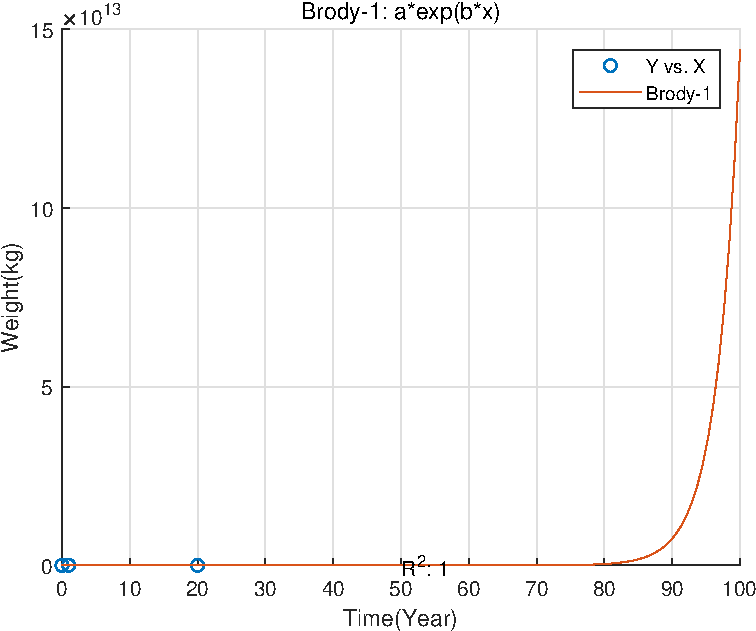
\includegraphics[width=.3\textwidth]{fit/Brody-1}}
  \subfigure[Brody-2]{\label{fig:Brody-2}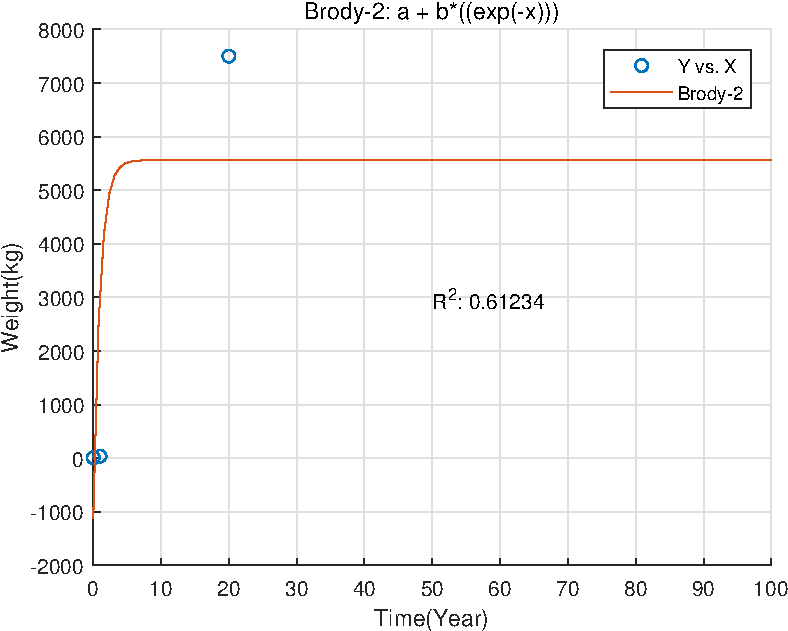
\includegraphics[width=.3\textwidth]{fit/Brody-2}}
  \subfigure[Bertalanffy]{\label{fig:Bertalanffy}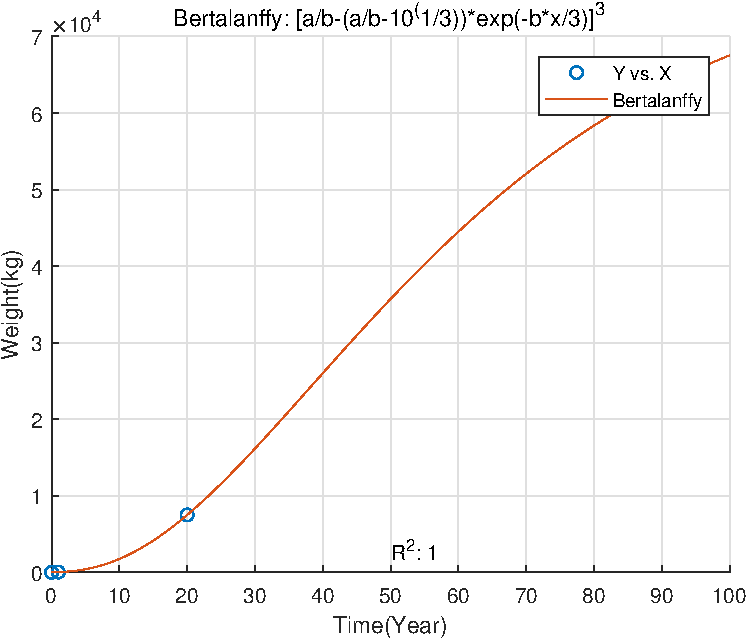
\includegraphics[width=.3\textwidth]{fit/Bertalanffy}} \\
  \subfigure[Gompertz]{\label{fig:Gompertz}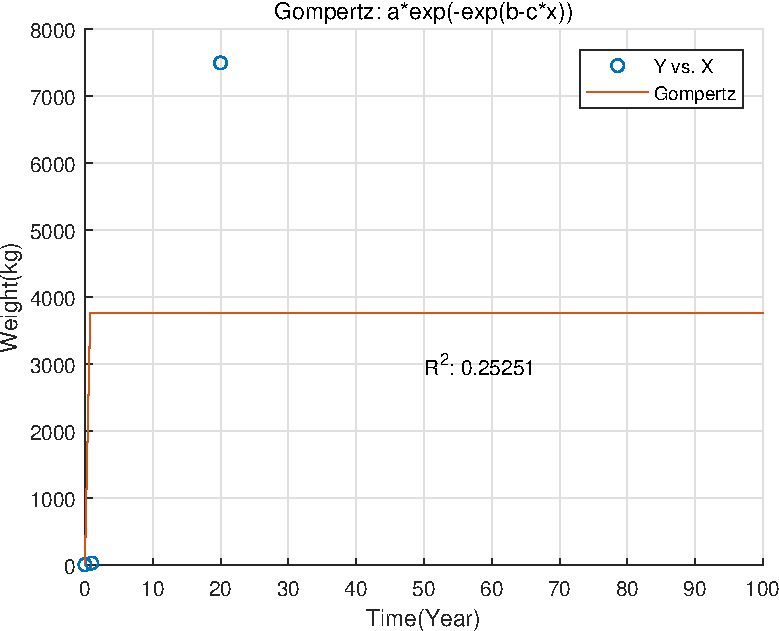
\includegraphics[width=.3\textwidth]{fit/Gompertz}}
  \subfigure[Janoschek]{\label{fig:Janoschek}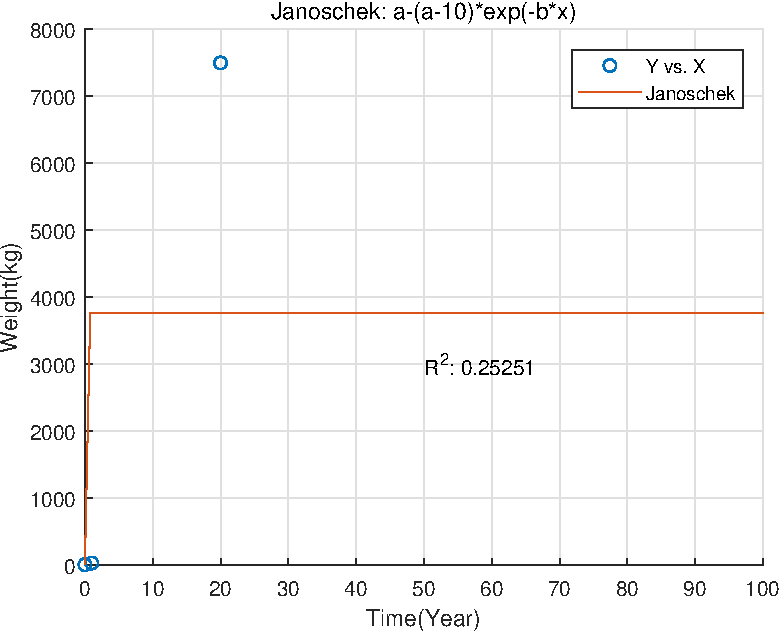
\includegraphics[width=.3\textwidth]{fit/Janoschek}} \\
  \subfigure[Logistic]{\label{fig:Logistic}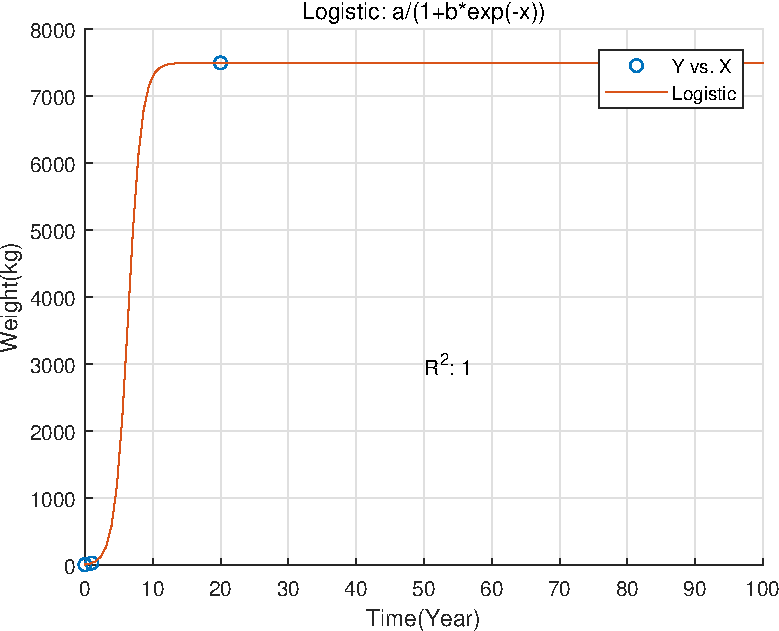
\includegraphics[width=.3\textwidth]{fit/Logistic}}
  \subfigure[Richards]{\label{fig:Richards}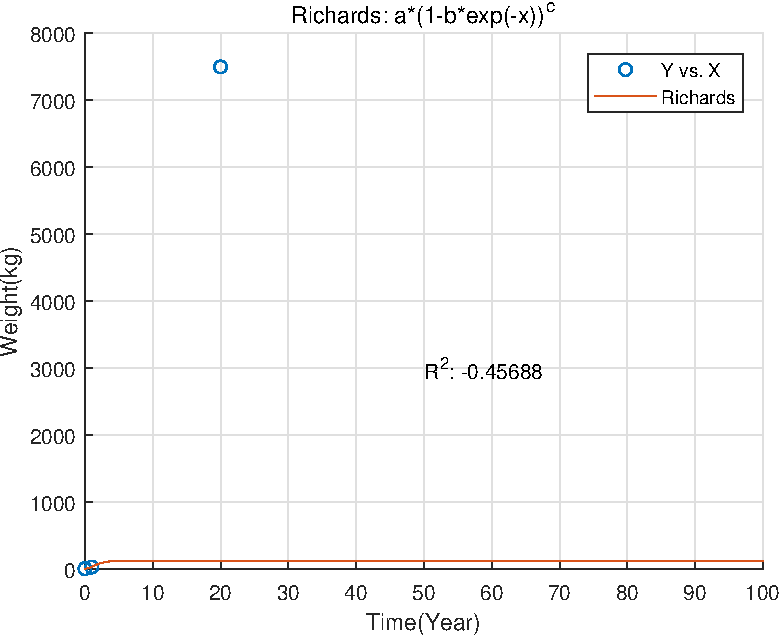
\includegraphics[width=.3\textwidth]{fit/Richards}}
\caption{Fitting the weight growth curve of the dragon}\label{fig:dragon-weight}
\end{figure}
After data substitution, figure \ref{fig:Logistic} is the most consistent with the actual situation.

\begin{figure}[htbp]
    \centering
    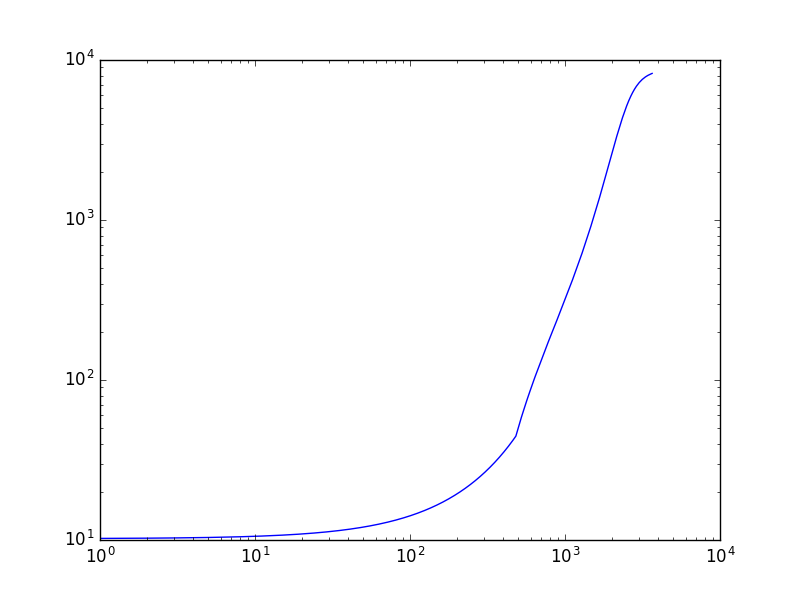
\includegraphics[width=.5\textwidth]{figures/attri/weight.png}
    \caption{Weight in the first 10 years , plotted on a logarithmic axis}
    \label{fig:weight}
\end{figure}

\subsection{Dragon's Energy Model}
    
\begin{defn}{Energy}
\end{defn}

Methane is a high-energy substance produced by the fermentation of carbohydrates in the feed in the rumen. Ruminants need to repeatedly absorb nutrients, and there are small peptides in the rumen, which promote the generation of gastric microorganisms, such as methanogens, which will decompose carbohydrates and generate methane.

The proportion of energy the animal consumes converted to methane: \cite{CH4proportion}
\begin{equation}\label{equ:甲烷转化率}
Y_m = 1.30+0.112D+L(2.37-0.050D)
\end{equation}

Daily methane emission from animals:

Consumption of energy: assuming that dragons are warm-blooded animals, the energy of maintenance, growth and activity can all refer to domestic cattle. The formula coefficient can be modified according to the actual data.\cite{consumption-energy}.
\begin{itemize}
    \item Net energy required for maintenance($NE_m$)
    \begin{itemize}
        \item Adult dragon: $0.299w^{0.75}\times A$.
        \item Growing dragon: $0.614w^{0.67}\times A$.
    \end{itemize}
    \item Net energy required for growth($NE_g$): $WG(1.5+0.045W)/(1-0.030WG)$. Ignore the adults.
    \item Net energy required for activity($NE_a$): \[NE_a=\int_0^{T_f}6.468\times\frac{A}{E}\,\D t.\]
    \item Net energy required for breathing fire($NE_h$): $0.7M\times 50.07$, take the calorific value of methane is $50.07MJ/kg$,take its combustion rate is 70\%.
    \item Daily energy intake(Suppose the energy conversion efficiency is 55\%).
    \[GE = \frac{NE_m+NE_g+NE_a+NE_f+NE_h}{0.55\times D\%}+SE.\]
\end{itemize}

\begin{figure}[t]
    \centering
    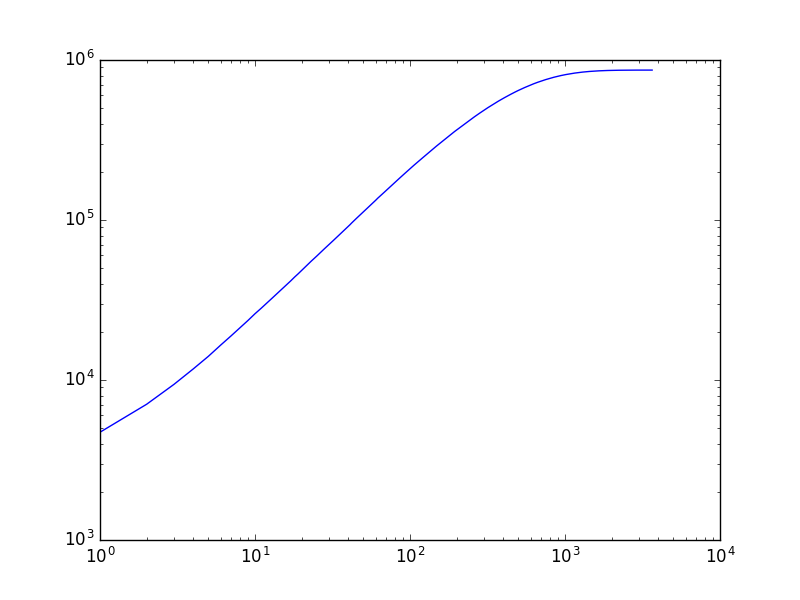
\includegraphics[width=.5\textwidth]{figures/attri/energy.png}
    \caption{Ground energy in the first year to the tenth year}
    \label{fig:energy}
\end{figure}

\subsection{Dragon's Mental State Model}

\begin{defn}{Mental State\footnote{Can be viewed as efficiency}}
\end{defn}
Denote as E
\begin{enumerate}[(1)]
    \item The efficiency of dragon is a number changing between $(0,1)$, which is related to its daily activities, and the independent variable is time.
    \item The efficiency of dragons affects the energy consumption of their daily activities. Specifically, the higher the mental state, the lower the energy consumption.
    \item The efficiency decay rate of the dragon is related to its age, that is, the older the dragon is, the slower its mental state consumption will be (reflected by the decrease of Q value).
    \item The dragon's energy should be independent of each other every day, and the energy should be restored to the threshold $E_0$ on the second day after sleeping every night (represented by the random number generated between $(0.9,1)$, indicating that the dragon's sleep is inconsistent every day, and the $E_0$ is high if the dragon sleeps well).
    \item The irregular work and rest of the dragon is reflected in the fact that when E decreases to a certain critical value (denoted as $E_f$), the dragon will start to rest, and when $E<E_f$, the dragon will stop moving.
\end{enumerate}

$E_f$ range reference $(0.1,0.15)$, we can get the figure \ref{fig:spirit} plotted.

    \begin{equation}\label{equ:精力E}
    E=E_0e^{-kt}
    \end{equation}
and the value Q is
    \begin{equation}\label{equ:Q值}
    Q=\frac{A}{1+Be^{CT}}
    \end{equation}
    \begin{itemize}
        \item $A$, $B$ and $C$ are constant in the equation\eqref{equ:Q值}, which should be determined according to the data
        \item $T$: the age of the dragon
        \item $t$: the time when the dragon is active after getting up, $t=2$ represents the second hour after getting up
        \item $T_f$: the moment when dragon mental state reaches the critical value
     \end{itemize}
     
\begin{figure}[htbp]
    \centering
    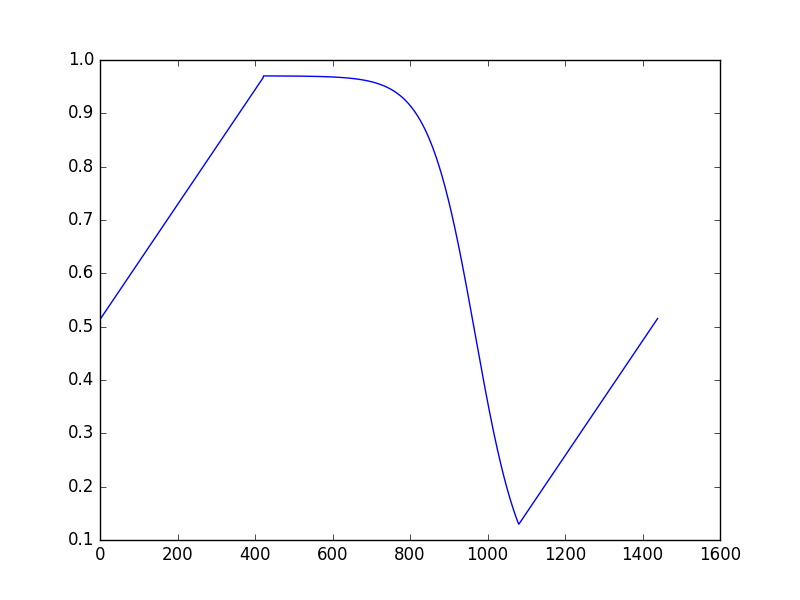
\includegraphics[width=.5\textwidth]{figures/attri/spirit.png}\\
    Gradual consumption in daytime, linear recovery at night
    \caption{Mental state -- efficiency }
    \label{fig:spirit}
\end{figure}

\subsection{Fly Model}
%飞行、喷火、防御

The flying process of the dragon is regarded as uniform motion, regardless of the influence brought by acceleration, temperature change, flying height and efficiency.


\subsection{Breath Fire Model}

1. The fire-breathing principle assumes that the rumen in the dragon body can decompose the cellulose in food to produce methane, which is stored in a certain organ in the body. When it is necessary to breathe fire, the methane will be transported to the lower jaw, and the flame will be ejected through ignition(To do this, it is also necessary to assume that the dragon's food contains green plants, otherwise cellulose cannot be obtained.).

2. The fuel consumption of the dragon does not consider the effect of efficiency.

The proportion of energy the animal consumes converted to methane: \cite{CH4proportion}
\begin{equation*}
Y_m = 1.30+0.112D+L(2.37-0.050D)
\end{equation*}

Feeding level calculation
\[
L=A\frac{NE_m+NE_g+NE_a+NE_f}{NE_m}
\]

 
Daily consumption of methane
\[
M = NE_m\frac{Y_m}{100}\times 0.3049
\]
    
\subsection{Resist Trauma Model}

As mentioned in the hypothesis, dragon scales are an important defense for dragons.Besides, the claws and wings of dragons are not only weapons of attack, but also means of defense.The dragon is able to withstand great trauma, and the dragon's ability to heal itself is also very strong.So unless it's a devastating injury, the dragon is essentially unaffected.

\subsection{Climatic Condition Simulation Model}

Note: Since the dragon's hard shell is not easy to be affected by external temperature, the direct impact of temperature on the life of the dragon is not discussed in this model (there is still an indirect impact).

\begin{defn}{Arid Region}
 Features: lack of water day and night, temperature difference, more sand, strong sunshine.
\end{defn}
\noindent
Impact on dragons:
\begin{enumerate}
    \item Windblown sand and sunshine hinder flight: appropriately increase the flight energy consumption coefficient and appropriately reduce the average flight speed $V$.
    \item Because of the hot environment and lack of water, the appetite and digestion level of the dragon are reduced: both the food energy $GE$ and the digestibility are reduced.
    \item As plants are scarce, dragons cannot get enough cellulose from their ingestion: proper reduction of the conversion rate of methane in $Y_m$ formula will indirectly reduce dragons' fuel consumption\footnote{The energy expended by breathing fire.}.
\end{enumerate}

\begin{defn}{Warm Temperate Region}
Features: comfortable climate, abundant resources.
\end{defn}
\noindent
Impact on dragons:
\begin{enumerate}[(1)]
    \item Due to the appropriate environmental conditions, the dragon's energy decline rate will slow down: the $K$ value\footnote{Maximum environmental capacity.} will be appropriately reduced.
    \item Adequate food sources: appropriately increase the dragon's food intake $GE$ and fecal mass $SE$.
\end{enumerate}


\begin{defn}{Arctic Region}
 Features: extremely low temperature, mostly Marine glaciers.
\end{defn}
\noindent
Impact on dragons:
\begin{enumerate}[1]
    \item Due to the extremely cold temperature and the decrease of food sources, it is considered to add the hibernation mechanism for dragons in this region (sleeping most of the time, the energy consumption for flight, activity and fire breathing is greatly reduced, but the energy consumption for growth and maintenance remains the same);Specifically, the dragon efficiency threshold is raised, and $E_f$ is modified to about 0.8 (that is, the daily rest time is greatly advanced, and the activity time is greatly reduced) : it is not necessary to be 0.8, and the ideal $E_f$ value should make the daily activity time about two to three hours.
    \item Due to hibernation, the daily flight time is greatly reduced, and the $T_f$ is adjusted to about 10min-30min.
    \item Because the temperature is too low, it has an inhibitory effect on the fire spraying effect of the dragon, and the emitted flame is weakened (the coefficient is reduced to 0.2-0.4 in the formula of the fuel consumption, that is, the combustion rate is $20\%$ to $40\%$).
    \item $GE$ energy intake should be reduced by the same proportion, that is, daily food intake should be reduced during hibernation.
\end{enumerate}

\subsection{Population and Community Model}

Next, we will discuss the impact of the addition of dragons on other populations in the environment.
\noindent
Note:
\begin{enumerate}[(1)]
    \item Since it is assumed that the dragon lives in a natural reserve (Yellowstone national park), its main food source should be cattle, sheep and other herbivores.
    \item Since it is assumed that the fire breathing principle of the dragon is that the body organs convert the ingested cellulose into methane, it is assumed that the dragon also feeds on grass in this setting.
\end{enumerate}

It is assumed that dragons mainly feed on cattle and sheep, and now we can explore its impact on the food chain (only the food chain including cattle and sheep is considered).

It is assumed that in the original environment:

producer A (green plant) 

consumer herbivore B (cattle and sheep)

now put dragon C is added to the food chain

The competitive relationship between cattle and sheep is not considered here, and it is regarded as the same category.


 .\phantom{Thisisaphantomspacemade}\xymatrix{
        & *+[F]{A}\ar@/_/[dl]\ar@/^/[dr] & \\
        *+[F]{B}\ar@/_/[rr] & & *+[F]{C}
    }
    
Before the dragon joined the food chain, A and B formed the standard predation model

 \begin{align}
    \diff{x}{t} &= (a-by)x \label{equ:标准捕食模型-1} \\
    \diff{y}{t} &= (nx-m)y \label{equ:标准捕食模型-2}
    \end{align}
By studying the orbits of the equations \eqref{equ:标准捕食模型-1} and \eqref{equ:标准捕食模型-2}, we can know the quantity change rule of A and B.

The equation set has two singularities $(0,0)$, $(m/n,a/b)$, and the value of the Jacobi matrix of the vector field of the equation set \eqref{equ:标准捕食模型-1} and \eqref{equ:标准捕食模型-2} at the singularities $(0,0)$ is
    \begin{equation}\label{equ:Jacobi矩阵-1}
    J = \begin{bmatrix} a-by & -bx \\ ny & nx-m \end{bmatrix}
      = \begin{bmatrix} a    & 0   \\ 0  & -m   \end{bmatrix}
    \end{equation}
The two eigenvalues of $J$ are $a>0$ and $-m<0$, so the singularity $(0,0)$ is the saddle point and unstable.

The value of the Jacobi matrix of the vector field of equations \eqref{equ:标准捕食模型-1} and \eqref{equ:标准捕食模型-2} at the singularity $(m/n,a/b)$ is
    \begin{equation}\label{equ:Jacobi矩阵-2}
    J = \begin{bmatrix} a-by & -bx   \\ ny    & nx-m \end{bmatrix}
      = \begin{bmatrix} 0    & -bm/n \\ na/b  & 0    \end{bmatrix}
    \end{equation}
The two eigenvalues of $J$ are imaginary $\pm i\sqrt{ma}$, so the singularity $(m/n,a/b)$ is the focal singularity.
The equation is reduced to first-order differential equations
    \begin{equation}\label{equ:一阶微分方程}
    (nx-m)y\,\D x = (a-by)x\,\D y
    \end{equation}
Equation \eqref{equ:一阶微分方程} is a variable separation equation with zero solutions($x=0$, $y=0$) and two semi-linear orbits
    \begin{equation*}
    \begin{cases}
    x=0, y>0 & \text{Rail line:} y=y_0e^{-mt} \\
    y=0, x>0 & \text{Rail line:} x=x_0e^{at}
    \end{cases}
    \end{equation*}
Separable variables
    \begin{equation}\label{equ:分离变量}
    \frac{(nx-m)\D x}{x} = \frac{(a-by)\D y}{y}
    \end{equation}
From the initial value $(x_0,y_0)$($\neq (0,0)$) to $(x,y)$, the definite integral of equation \eqref{equ:分离变量} is made to obtain the integral curve passing through $(x_0,y_0)$
    \begin{equation}\label{equ:积分曲线}
    -m\ln\left(\frac{x}{x_0}\right)+n(x-x_0) = a\ln\left(\frac{y}{y_0}\right)-b(y-y_0)
    \end{equation}
Take the exponent of the equation \eqref{equ:积分曲线}
    \begin{equation}\label{equ:积分指数1}
    y^ae^{-by}x^me^{-nx} = K
    \end{equation}
Where K is a constant
    \begin{equation}\label{equ:积分指数2}
    K=y_0^ae^{-by_0}x_0^me^{-nx_0}
    \end{equation}
Note that
    \begin{equation}\label{equ:函数f}
    f(x)=y^ae^{-by}
    \end{equation}
    \begin{equation}\label{equ:函数g}
    g(x)=x^me^{-nx}
    \end{equation}
    
The differential method tells us that $f(x)$ is a unimodal function, which gets the maximum at the focal ordinate $y=a/b$, and gets the minimum 0 for $y=0$ and $y=+\infty$. $f(y)$ increases from 0 strictly monotone to the maximum on the interval $[0, a/b]$, and decreases strictly monotonically and approaches 0 on the infinite interval $y>a/b$.

In the same way, $g(x)$ is a unimodal function, which gets the maximum at the focal abscissa $x=m/n$, and gets the minimum 0 for $x=0$ and $x=+\infty$.$g(y)$ increases from 0 strictly monotone to the maximum on the interval $[0, m/n]$, and decreases strictly monotonically and approaches 0 on the infinite interval $x>m/n$.

So the K in the equation \eqref{equ:积分指数2} has to satisfy the following inequality
    \begin{equation}\label{equ:不等式}
    0 \leq K \leq \frac{a^am^me^{-a-m}}{b^an^m} =: K_0.
    \end{equation}
Through the above fact is easy to know when the equation \eqref{equ:积分指数1} in the $K$ value $(0, K_0)$, the corresponding orbit type is surrounded by a focal point singularity $(m/n, a/b)$ closed track. Therefore, the equations of singular point $(m/n, a/b)$ is the center. In the first quadrant center filled with surrounded around the center of closed track. This shows that when the initial values $x_0$ and $y_0$ are greater than 0, a and b are not extinct, and their number is cyclical change. See below:
    \begin{figure}[ht]
        \centering
        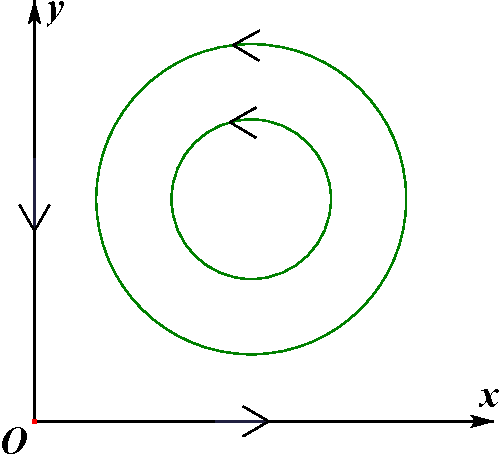
\includegraphics[width=.5\textwidth]{dragon-period.pdf}
        \caption{Periodic change}\label{e-fig:周期性变化}
    \end{figure}
After dragon C joins the food chain, the model becomes (in this model, the number of dragons is constant to three, regardless of the change in the number of dragon population)
\begin{align}
    \diff{x}{t} &= (a-by-c)x \label{equ:标准捕食模型-3} \\
    \diff{y}{t} &= (nx-m-p)y \label{equ:标准捕食模型-4}
    \end{align}
There will be two situations:

1. The environmental carrying capacity cannot meet the growth needs of the dragon, that is, $a<c$ in equation \eqref{equ:标准捕食模型-3} and $nx-m-p<0$ in equation \eqref{equ:标准捕食模型-4}. At this time, A will decrease in quantity at a slower and slower speed until extinction, and B will also face extinction.(in this process, if either A or B dies out first, the c and p in equation \eqref{equ:标准捕食模型-3} and equation \eqref{equ:标准捕食模型-4} will increase correspondingly (depending on the predation of the dragon).)

2. Environmental capacity can support the growth of the dragon, the equivalent of in equation \eqref{equ:标准捕食模型-1} and equation \eqref{equ:标准捕食模型-2}, will decrease $a$ and increase $m$, at this point A and B number was still above similar cyclical change, but the overall produce translation (translational direction according to the condition of feeding of the dragon, that is, the relative size of $c$ and $p$ in the equation \eqref{equ:标准捕食模型-3} and equation \eqref{equ:标准捕食模型-4}.)





\subsection{Migration Model}

A program simulation is used to simulate the migration of dragons. The simulation program depends on the establishment of the model. It follows the diffusion path of finance by adjusting its movements according to its environment and energy density, while its interactions are determined by internal properties such as distance and speed.

After several simulations, we obtain the trajectories of several dragons. The confidence interval of 95\% was calculated by statistical model as the survival area of the dragon.

Finally,we obtain that the living space a dragon needs is \emphb{824}$km^2/day$

\begin{figure}[htbp]
    \centering
    \subfigure[The 100-year migration route]{\label{fig:mig-way}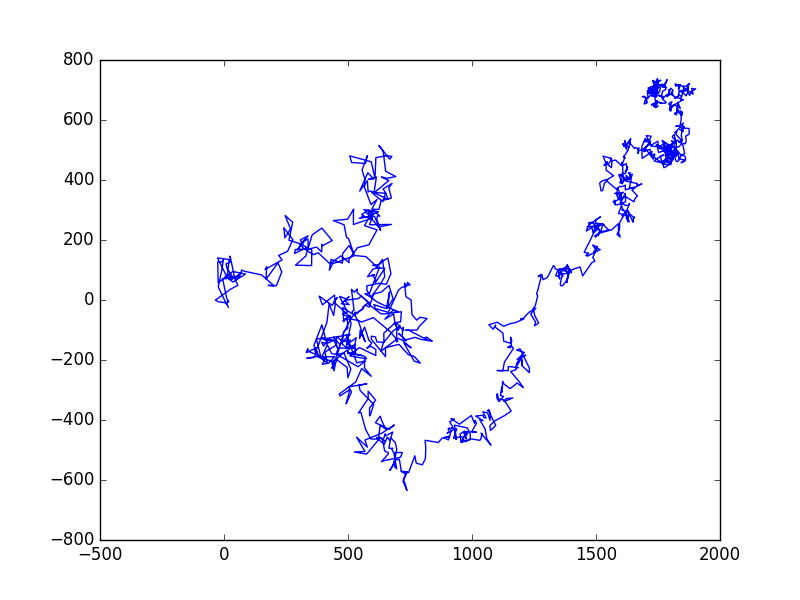
\includegraphics[width=.45\textwidth]{figures/migration/way.png}}
    \subfigure[Environmental energy density for one year]{\label{fig:mig-env}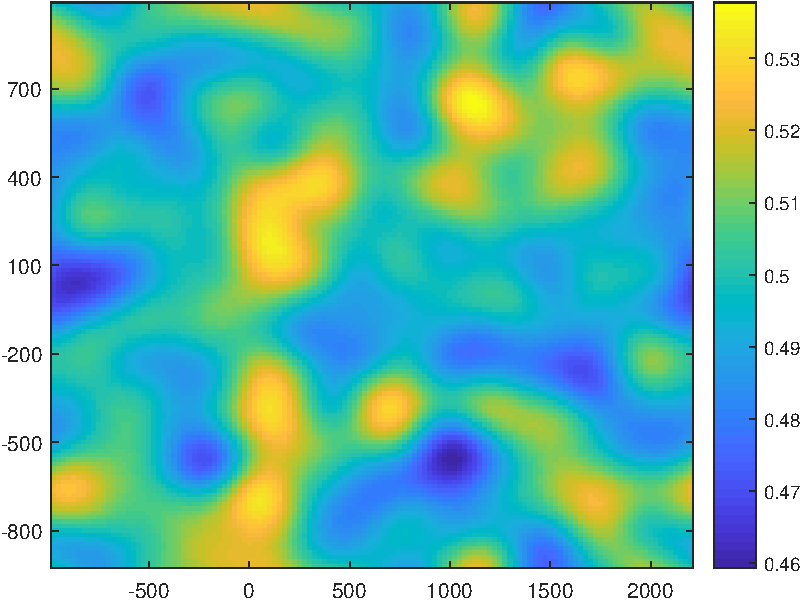
\includegraphics[width=.45\textwidth]{figures/migration/env.pdf}}
    \caption{For one dragon}
    \label{fig:100年迁移}
\end{figure}

\begin{figure}[htbp]
    \centering
    \subfigure[The 10-year migration route for 3 dragons]{\label{fig:mig-way-2}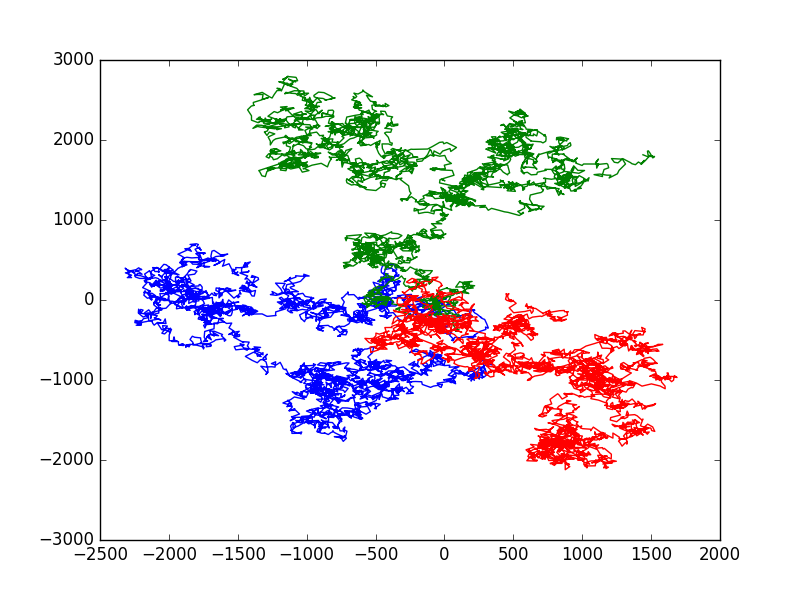
\includegraphics[width=.45\textwidth]{figures/interact/way.png}}
    \subfigure[Environmental energy density for one year]{\label{fig:mig-env-2}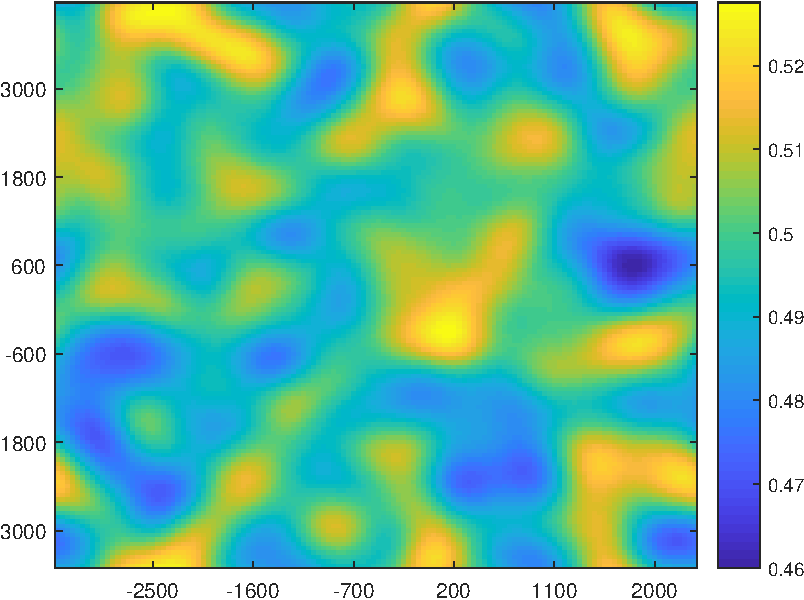
\includegraphics[width=.45\textwidth]{figures/interact/env.pdf}}
    \caption{For three dragons}
    \label{fig:3条龙}
\end{figure}



\section{Extended Model Application}

\subsection[Dragon Survival Needs Model]{Dragon Survival Needs Model(Under Different Climatic Conditions)}

Next, we will answer that how large a community is necessary to support a dragon for varying levels of assistance that can be provided to the dragon.At the same time, we take climate into account.

Suppose that only 2\% of the energy (GE) a dragon gets from food per day comes from plants (used only to obtain the methane that provides the basis for the fire) : based on the previous calculation, a dragon needs to eat vegetables per day

\[X_0=\frac{2\%GE}{0.00557} \times 0.1 kg\]

(we know that 100g vegetables -- 13.3 kilocalorie -- 0.0557MJ\cite{food1})

Take the standard body weight of the adult dragon is 8t, and solve for $X_0=808.26kg$.

The rest of the food for cattle, sheep and other herbivores.Assume they are all mountain goat: according to the average weight of the goat--32kg \cite{food2}, 203 kilocalorie per 100g of mutton ($\approx 0.84854MJ$)

According to the previous calculation, the number of sheep the dragon needs to feed on per day is (unit: one)

\[Y_0=98\%GE \times\frac{100}{32 \times 1000 \times 0.84854 \times 60\%}\]

Take the standard weight of the adult dragon is 8t, to solve for $Y_0=13.54$. An adult dragon approximately eats 13.54 mountain goats per day. 

In the exposition of the ecological impact of dragons, it has been discussed that the environmental carrying capacity is not enough to support the survival of dragons.We will now discuss only the environmental support necessary for a dragon to live a stable life.

According to the daily activity area of the dragon mentioned above, the population density of mountain goats can be estimated to be at least

\[\rho_0=\frac{Y_0}{B\%\times S}\]

B is the predation rate of the dragon (1-10 is preferable, because the dragon do not eat every sheep in its range and will not eat again when they are full. In this model, we take B=3)

Take the adult dragon standard weight is 8t, and get $\rho_0$=0.548 (one/$km^2$)

Now we will consider the climate change, the local community support changes that occur when dragons migrate to different areas.First, according to the description of the effect of the climate on the dragon, after reasonably modifying the coefficient, draw the corresponding contrast chart (the contrast between the image in the climate and the initial image).Then the change of population support to the dragon was discussed according to three typical climates.

The arid region:Take the standard weight of the adult dragon is 8t, to solve for $X_0=673.44kg$, $Y_0=11.02$, $\rho_0$=0.446 (one/$km^2$)

The warm temperate region: Take the standard weight of the adult dragon is 8t, to solve for $X_0=904.87kg$, $Y_0=15.08$, $\rho_0=0.623$

The Arctic region:Because of the diversity of life in the polar regions, it is no longer possible to assume that the dragon feeds on vegetables and goats.The plants in the polar regions are mainly lichens and mosses. It is assumed that the dragons in the arctic get cellulose by eating mosses, and the main food is cod.

\begin{itemize}
    \item 100g moss -- 8 kilocalorie -- 0.03349MJ \cite{food1}
    \item 100g cod -- 78 kilocalorie -- 0.3265MJ \cite{food2}
\end{itemize}
\begin{align*}
X_0 &=\frac{2\%GE}{0.03349} \times 0.1 kg \\
Z_0 &=98\%GE \times\frac{0.1}{0.3265 \times 90\%} \\
\rho_0&=\frac{Z_0}{B\%\times S} \\
\end{align*}
Take the standard weight of the adult dragon is 8t, to solve for $X_0=305.32kg$, $Z_0=255.92kg$, $\rho_0$=10.358 (kg/$km^2$)

\begin{figure}
    \centering
    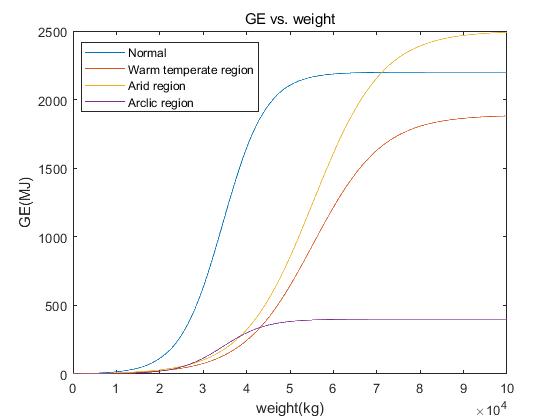
\includegraphics[width=.5\textwidth]{final/final2.png}
    \caption{Weight comparison in different environments}
    \label{fig:diff_env_weight}
\end{figure}

\begin{figure}
    \centering
    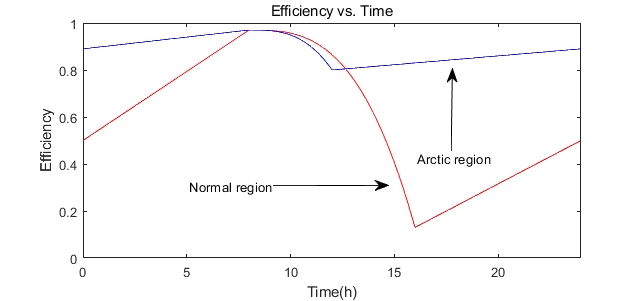
\includegraphics[width=.5\textwidth]{final/final3.png}
    \caption{Efficiency in different environments}
    \label{fig:diff_env_spirit}
\end{figure}

\subsection{Dragon Living Space Model}

Next, solve the problem of living space.Based on the model mentioned above, we can first calculate the living space required by a dragon.

\begin{figure}[h]
    \centering
    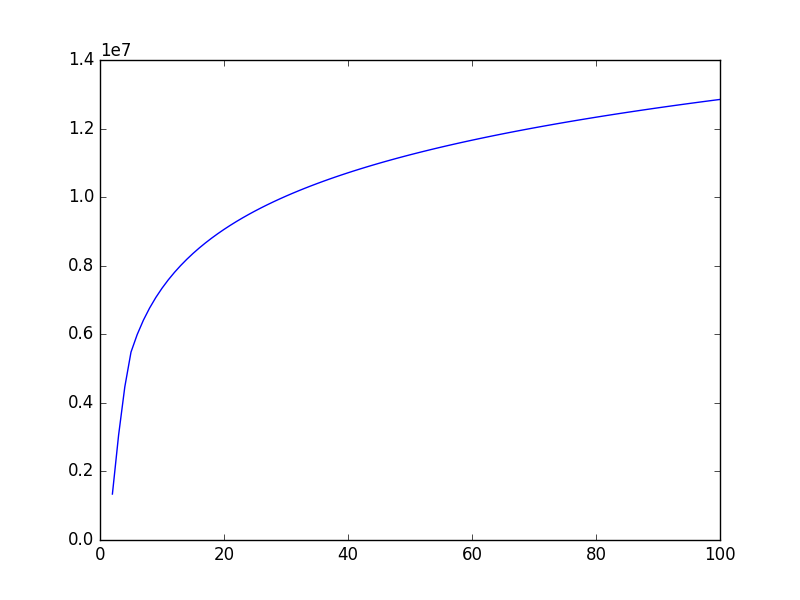
\includegraphics[width=.5\textwidth]{analysis/area.png}\\
    The x-coordinate is the number of years and the y-coordinate is the area($km^2$).
    \caption{The range of a dragon over time}
    \label{fig:area}
\end{figure}

In solving the problem of dragon living space, we also innovatively explored the interaction between multiple dragons and the attraction between dragons of the opposite sex.

\begin{figure}[htbp]
    \centering
    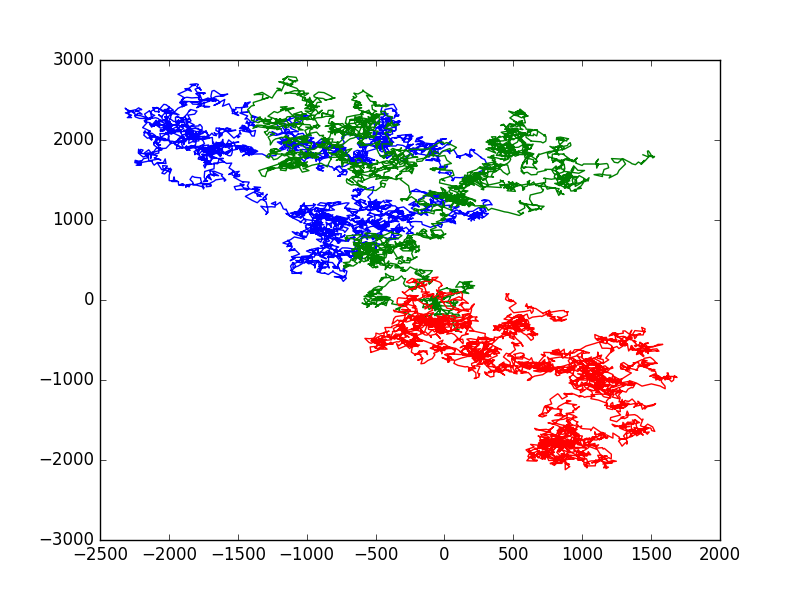
\includegraphics[width=.5\textwidth]{interact/way110.png}
    \caption{Interactions between dragons of the opposite sex}
    \label{fig:110}
\end{figure}

\begin{figure}[htbp]
    \centering
    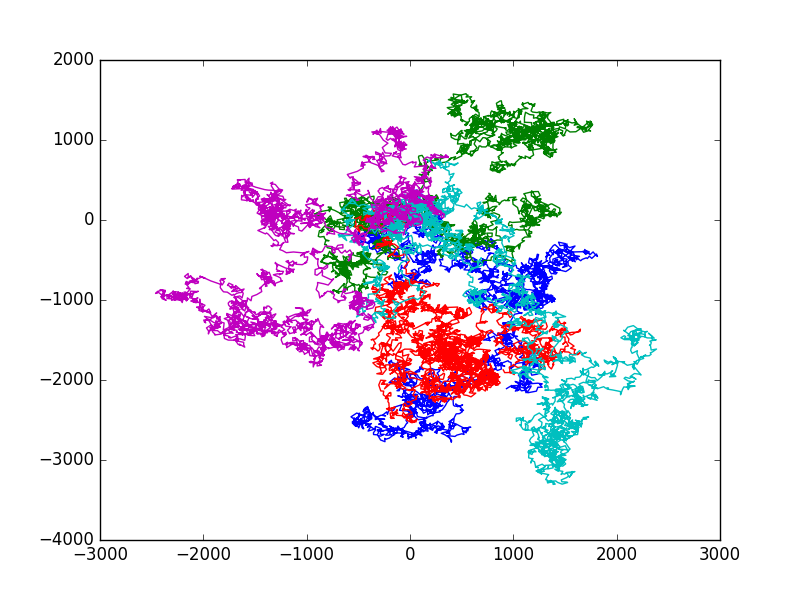
\includegraphics[width=.5\textwidth]{interact/way5.png}
    \caption{The interaction of five dragons}
    \label{fig:five-dragon}
\end{figure}

Finally,we obtain that the living spaces 3 dragon need is \emphb{$2.12\times 10^7$}$km^2/100years$

\section{Testing the Model}
\subsection{Sensitivity analysis}
Dragon for fictional creatures, different of the film and television works books on it, so in a slightly different parameter values. Such as the weight, said a year after their birth weight in the title for 30--40 kg, and the definition of adult is not clear, so use logistics model for regression analysis of the difference is larger, the late weight may come in and go out. But they are consistent, increase first and then decreases to zero, flight properties such as energy consumption will be affected by the corresponding, but the influence of proportion was only amplified. Therefore, you can set the scaling factor to make the result consistent.As shown in figure \ref{fig:test_model}.

\begin{figure}[htbp]
    \centering
    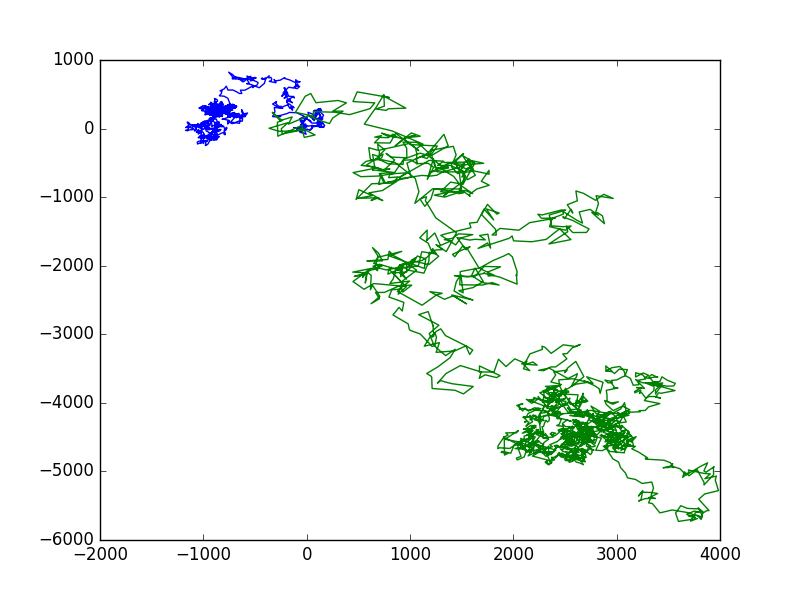
\includegraphics[width=.5\textwidth]{analysis/test_the_model.png}
    \caption{Sensitivity analysis}
    \label{fig:test_model}
\end{figure}

However, if the selection of the scaling factor is inconsistent, the body weight will also be affected. Thus affecting the flight speed, and the flight speed will affect the flight distance. So the range suitable for the survival of the dragon will be increased by the same proportion, and the results are different.

\subsection{Stability test}
To consider the actual situation of the random events, the impact of parameters using random variables instead of dragon behaviour, such as climate and energy density distribution. So the model results depends on the random number enough ``random''. For example, using C++ standard library random number by default engine, every time is to run the program results are the same, and the analysis of the model is not enough. The use of linear congruence, the number of seconds to will as simulated too fast lead to the change of a single period of time, is not conducive to simulate the actual situation.Therefore, in order to ensure the stability of the model, it is necessary to select an appropriate random number generation algorithm.The program USES an unsigned mason rotation generator that relies on nanoseconds.


\section{Conclusions}

By establishing basic models, we got a lot of valuable data, such as the ecological demand of the dragon: 13.54 sheep/day, 808.26kg of vegetables/day. The population density of sheep was $0.548 /km^2$.

The ecological impact of dragons is a problem within the planning. We made assumptions about the energy demand based on the data of raptors. The region where the dragon lives can provide different levels of help to the dragon. Collect regional information, and use the method of dimensionality reduction to classify different regions. We have also expanded from one dragon to many, taking into account the impact of different climatic regions. The living space a dragon needs is 824$km^2/day$. Moreover, the interaction between dragons is studied innovatively, considering the competition between dragons and the attraction between dragons of the opposite sex.

The migration of the dragon is an important part of the survival of the species. Multivariate analysis is used to determine the ecological factors between different environments. The impact of the change can be determined by establishing a corresponding analysis between the migration of the dragon and the resources needed for its growth.

\section{Strengths and Weaknesses}
\emphb{Strengths}
\begin{enumerate}
    \item The model is practical, the hypothesis is reasonable and the data can be checked.The hypothesis is to refer to the original work and some film and television works, and start from the animals that can be contacted in life. The data is easy to collect and conforms to the biological principle.
    \item The model is comprehensive.The coupling relationship is simplified and the simulation optimization is improved as simple as possible.
    \item Clean Architecture, strong expanding, strong commonality. With TDD, any development node can come up with a product that can be used, containing a few bugs, has certain functions and can be released.It was transplanted from Python to C++ in a mixed way, without loss of extensibility and obvious efficiency. It simulated three dragons in 100 years in less than one minute.
\end{enumerate}
\noindent
\emphb{Weaknesses}
\begin{enumerate}
    \item The model has made reasonable approximation in large scale for efficiency, but the simulation will cause large deviation after more than 100 years. And the API needs to be modified again to achieve the required accuracy.
\end{enumerate}















